\documentclass[justified]{tufte-handout}
\usepackage{../braph2_tut}
%\geometry{showframe} % display margins for debugging page layout

\title{Pipeline for Comparison of Connectivity-Functional Multiplex Data using Weighted Undirected graphs}

\begin{document}

\maketitle

\begin{abstract}
\noindent
This tutorial is not ready. You can find a similar one in CON BUT (\url{https://github.com/softmatterlab/BRAPH-2-Matlab/blob/develop/tutorials/pipelines/tut_a_con_but/tut_a_con_but.pdf}).
\end{abstract}

\fig{marginfigure}
	{fig:01}
	{
	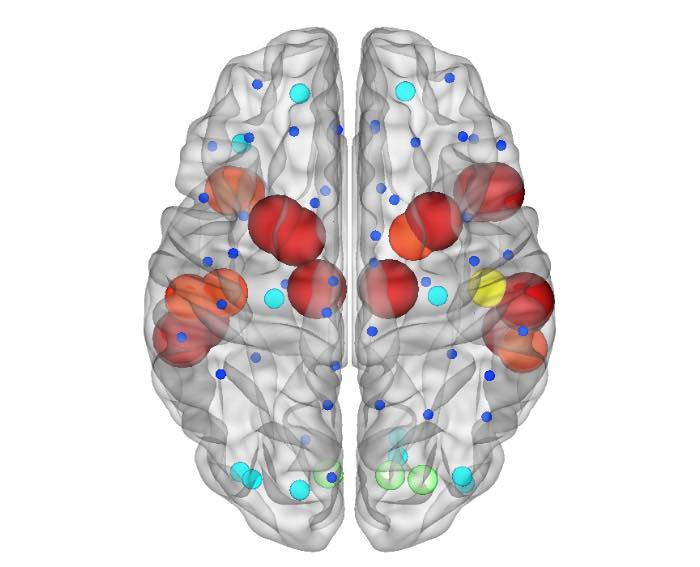
\includegraphics{fig01_01.jpg}
	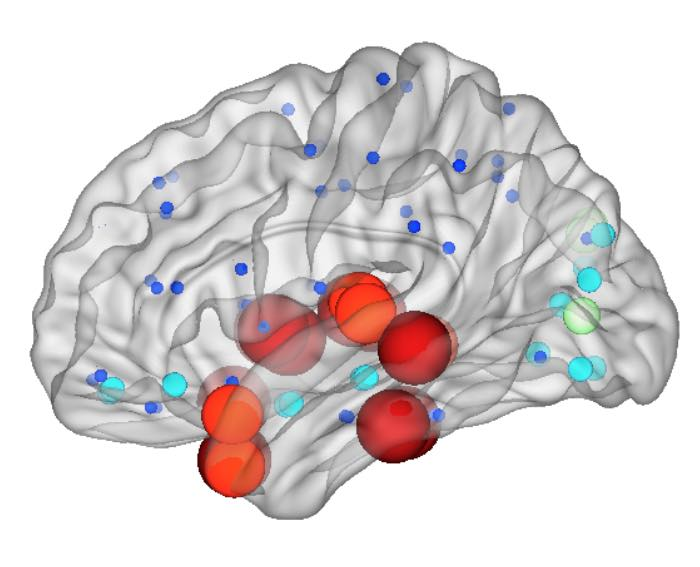
\includegraphics{fig01_02.jpg}
	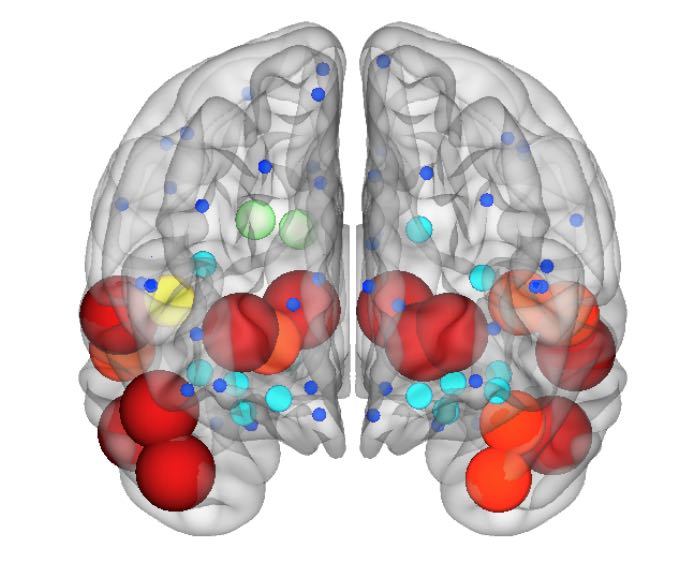
\includegraphics{fig01_03.jpg}
	}
	{Figure examples}
	{
	Examples of displays of \fn{Community Structure} with connectivity data binarized at fixed thresholds obtained using BRAPH 2.
	}
	
\tableofcontents

\clearpage
\section{Generate Example Data}

You can generate the example data by typing in the command line the instruction in \Coderef{cd:generate}.
%
\begin{lstlisting}[
	label=cd:generate,
	caption={
		{\bf Command to generate example data.}
		Command to generate the example data for connectivity and functional multiplex analyses. They will be placed in the folder \fn{./braph2/pipelines/connectivity-functional multiplex/Example data CON\_FUN\_MP XLS}, and include the brain atlas \fn{atlas.xlsx}, two folders (one for the connectivity data and the other for the functional data) with two folders with the subject files (\fn{CON\_Group1\_XLS} and \fn{CON\_Group2\_XLS} for the connectivity data, and \fn{FUN\_Group1\_XLS} and \fn{FUN\_Group2\_XLS} for the functional data), and the associated covariates files (\fn{CON\_Group1\_XLS.vois} and \fn{CON\_Group2\_XLS.vois} at the connectivity data, and \fn{FUN\_Group1\_XLS.vois} and \fn{FUN\_Group2\_XLS.vois} at the functional data). The details about the format of these files can be found in the tutorials \href{https://github.com/braph-software/BRAPH-2/tree/develop/tutorials/general/tut_ba}{Brain Atlas}, \href{https://github.com/braph-software/BRAPH-2/tree/develop/tutorials/general/tut_gr_con_fun_mp}{Group of Subjects with Connectivity-Functional Multiplex Data}.
	}
]
test_CombineGroups_CON_FUN_MP
\end{lstlisting}

\section{Open the GUI}

The general GUI of BRAPH 2.0 can be opened by typing \code{braph2} in MatLab's terminal. This GUI allows you to select a pipeline, in this case, \emph{Pipeline Connectivity-Functional Multiplex Comparison WU}, as shown in \Figref{fig:02}.

\fig{figure}
	{fig:02}
	{
	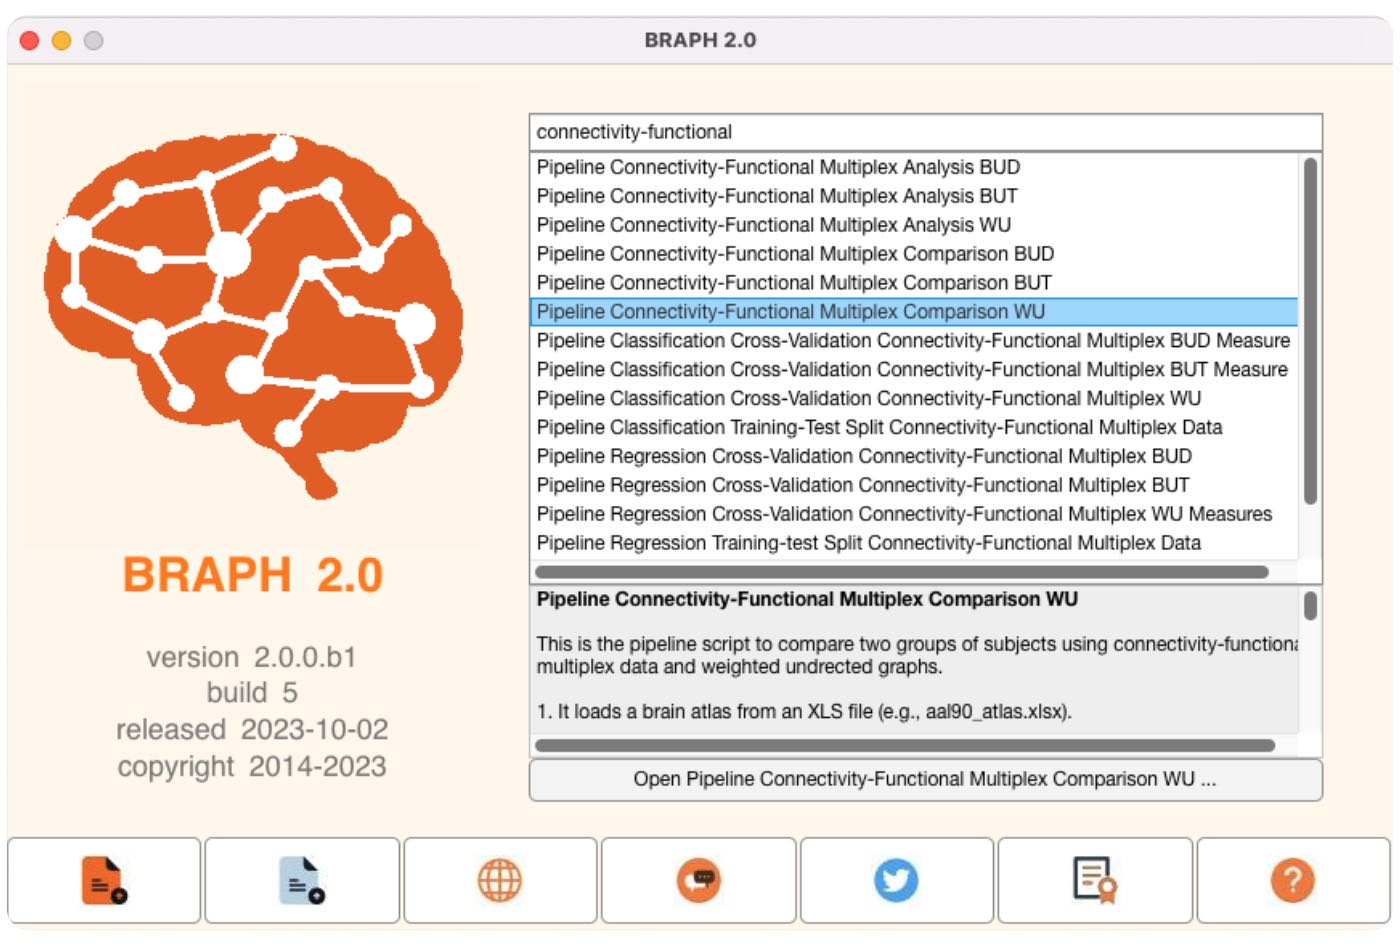
\includegraphics{fig02.jpg}
	}
	{BRAPH 2 main GUI}
	{
	BRAPH 2 main GUI with the pipeline \emph{Pipeline Connectivity-Functional Multiplex Comparison WU} selected.
	}

\begin{tcolorbox}[
	title=Pipeline launch from command line
]
To open the GUI and upload the connectivity-functional multiplex comparison pipeline, you can also do it from the command line by typing the commands in \Coderef{cd:launch}.
%
\begin{lstlisting}[
	label=cd:launch,
	caption={
		{\bf Code to launch the GUI to upload a pipeline file to compare two groups of subjects.}
		This code can be used in the MatLab command line to launch the GUI to upload a pipeline file.
	}
]
im = ImporterPipelineBRAPH2( ...
	'FILE', which('pipeline_connectivity_functional_multiplex_comparison_wu.braph2') ...
	);
pip = im.get('PIP');

gui = GUIElement('PE', pip, 'WAITBAR', true); gui.get('DRAW')
gui.get('SHOW')
\end{lstlisting}
\end{tcolorbox}

Once the pipeline is uploaded, you can see a GUI that contains different steps to: upload a brain atlas, upload the connectivity and functional multiplex data of two groups, analyze them, and finally, compare the groups (\Figref{fig:03}). 

\fig{marginfigure}
	{fig:03}
	{
	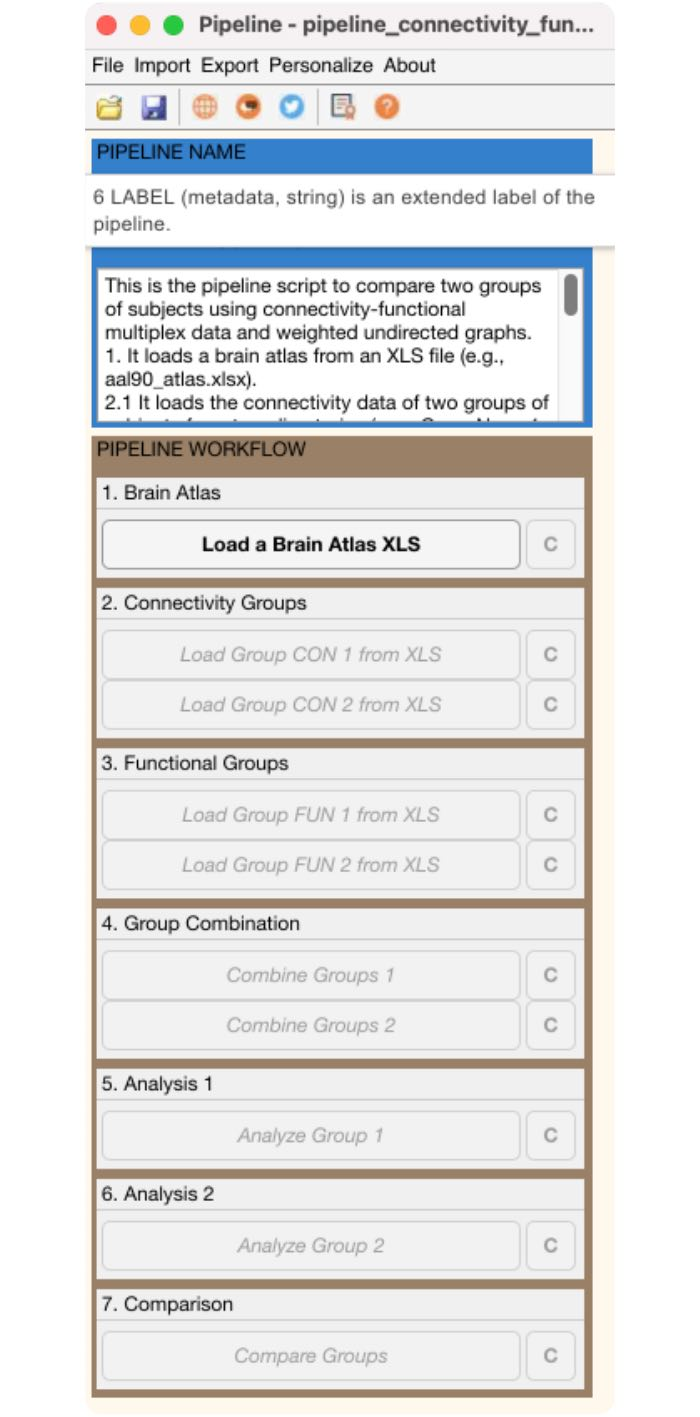
\includegraphics{fig03.jpg}
	}
	{Pipeline steps}
	{
	These are the steps of the pipeline. Only the first step is active when the pipeline is first opened. Subsequent steps will become active sequentially.
	}

\clearpage
\section{Step 1: Load the Brain Atlas}

\Figref{fig:04} shows how to upload and plot the brain atlas that you used to extract the \emph{connectivity-functional multiplex data} for your analysis. For more information on where to find different atlases or how to change plotting settings on the brain surface, check the tutorial \href{https://github.com/braph-software/BRAPH-2/tree/develop/tutorials/general/tut_ba}{Brain Atlas}.

\fig{figure*}
	{fig:04}
	{
	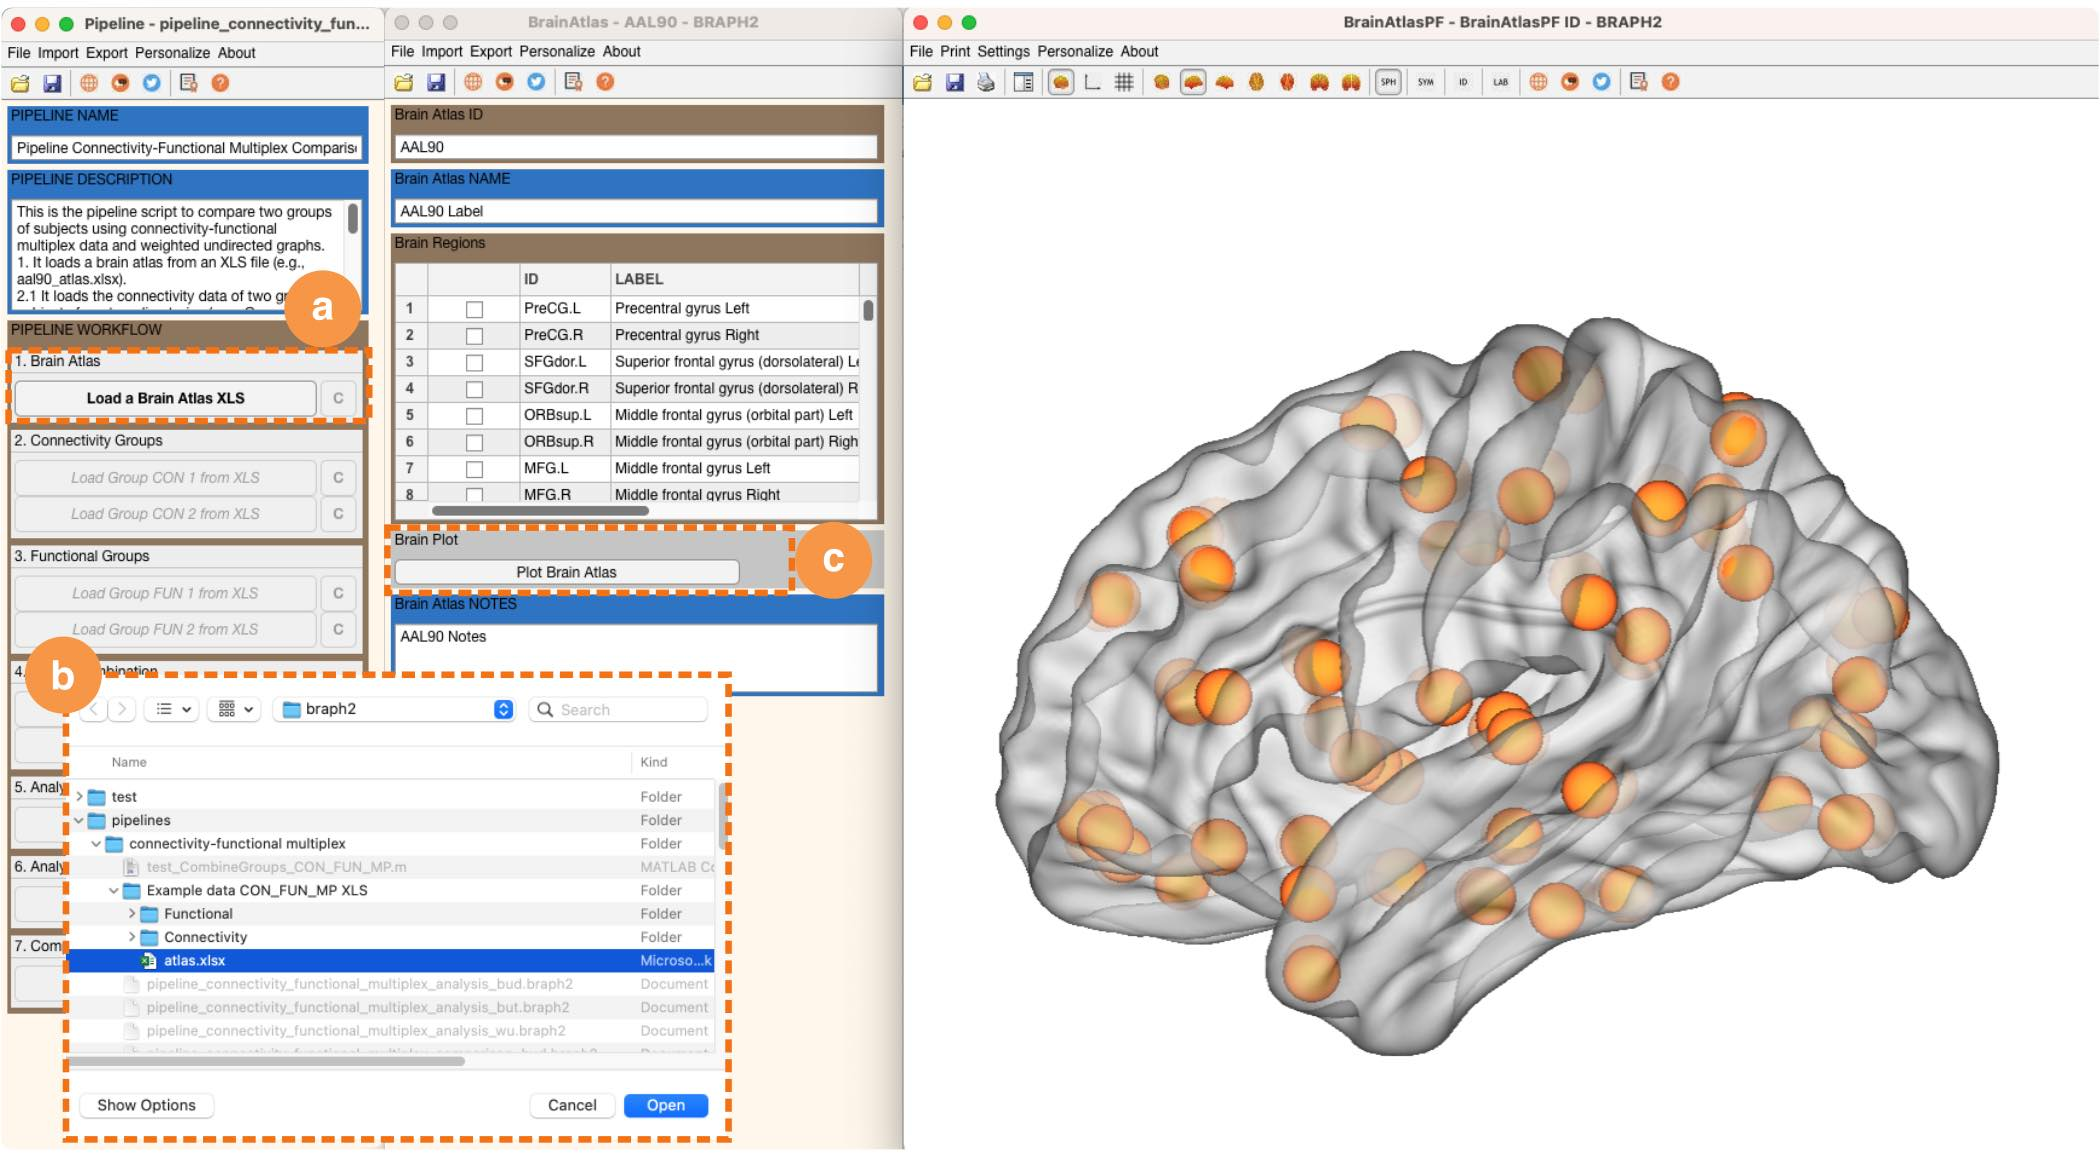
\includegraphics{fig04.jpg}
	}
	{Uploading the Brain Atlas}
	{
	Steps to upload the brain atlas:
	{\bf a} Click on \fn{Load Atlas} from the pipeline GUI.
	{\bf b} Navigate to the BRAPH~2.0 folder \fn{pipelines\_connectivity-functional multiplex\_Example data CON\_FUN\_MP XLS}, and select the atlas file, in this example the \fn{atlas.xlsx}.  
	{\bf c} You can visualize the brain atlas by pressing \fn{Plot Brain Atlas}. 
	}
 
\clearpage
\section{Step 2: Load the Connectivity-Functional Multiplex Group Data}

After you loaded the brain atlas, you can upload the \emph{connectivity data} for each group and later the \emph{functional data} for each group, as shown in \Figref{fig:05}. A new interface will be shown containing the data for the group you just selected. You can open each subject’s data by selecting the subject, right click, and select “Open selection” (for more information check the tutorial \href{https://github.com/braph-software/BRAPH-2/tree/develop/tutorials/general/tut_gr_con_fun_mp}{Group of Subjects with Connectivity-Functional Multiplex Data}).

\fig{figure}
	{fig:05}
	{
	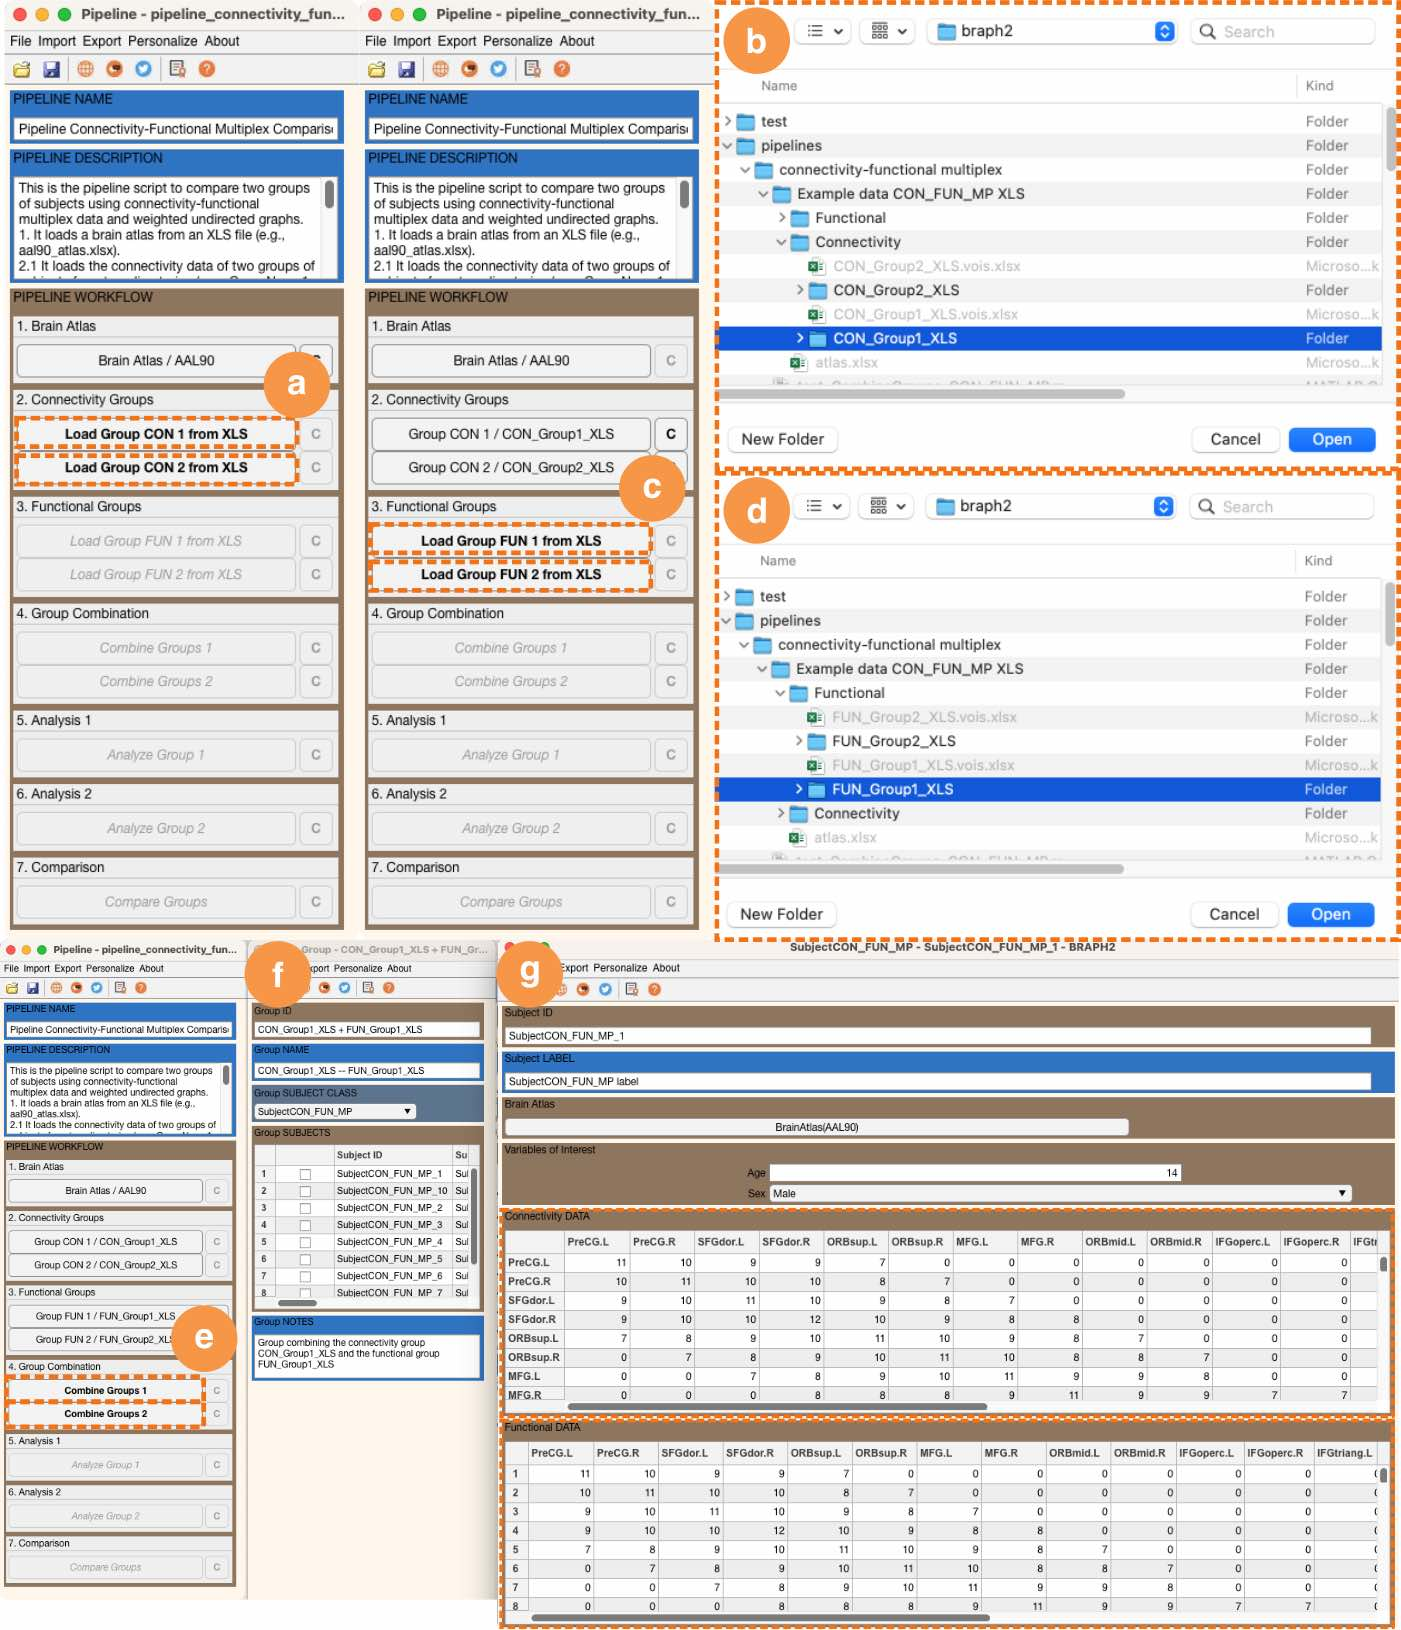
\includegraphics{fig05.jpg}
	}
	{Loading and visualizing the group data}
	{
	{\bf a} From the pipeline GUI, click on \fn{Load Group CON 1 from XLS} and \fn{Load Group CON 2 from XLS} to load the connectivity data of both groups.
   	{\bf b} Navigate to the BRAPH~2.0 folder \fn{pipelines}, \fn{connectivity-functional multiplex}, \fn{Example data CON\_FUN\_MP XLS}, \fn{connectivity}, and select the group folder that you want to upload. 
        {\bf c} Once the connectivity data is uploaded, click on \fn{Load Group FUN 1 from XLS} and \fn{Load Group FUN 2 from XLS} to load the functional data of both groups.
   	{\bf d} Navigate to the BRAPH~2.0 folder \fn{pipelines}, \fn{connectivity-functional multiplex}, \fn{Example data CON\_FUN\_MP XLS}, \fn{functional}, and select the group folder that you want to upload. 
   	{\bf e} After uploading the data for both modalities, click on \fn{Combine Groups 1} and \fn{Combine Groups 2} to create groups with connectivity-functional multiplex subjects, and it will open a window for group 1 {\bf f}  and a window for group 2 {\bf g}.
	}
 
\clearpage
\section{Step 3: Analyzing the Data of Group 1}

Once you have loaded the data for both groups, you can begin analyzing the data for the first group by clicking on \fn{Analyze Group 1} (\Figref{fig:06}a). 
This will open a new interface called \fn{Analyze Ensemble}, which allows you to calculate and visualize graph measures for the first group. 
Before these network measures are calculated, it is important to ensure the following things: 
\begin{enumerate}
	\item The analysis parameters are set correctly (e.g., the thresholds).
	\item The graph parameters are set correctly.
	\item The measures are configured with the parameters you desire (note that not all measures have parameters).
\end{enumerate}

Importantly, the parameters you select at the beginning will remain fixed for the rest of the pipeline (including the analysis of the second group and the comparison between groups). We will now guide you through the process of preparing these parameters for both measures and graphs. It is important to keep in mind that the default parameters should work well for most cases.

\subsection{Setting Analysis Parameters}

In the \fn{Analyze Ensemble} interface, you can configure the analysis parameters (\Figref{fig:06}b).
In the \code{REPETITION TIME [s]} section, you can include the repetition time with which your images were acquired, for example, to analyze the data only within a fraction of the repetition time.
In the \code{MIN FREQUENCY [Hz]} and \code{MAX FREQUENCY [Hz]}, you can edit the values to analyze your data within a certain frequency band such as in the case of EEG or MEG data.
In the \code{CORRELATION RULE}, you can select the type of correlation you want to run using the brain activation signals between brain areas. 
Finally, in the \code{NEGATIVE WEIGHTS RULE}, you should decide if you want to set the negative weights to zero, their absolute values or exclude them from the analysis since graph theory measures are not defined for negative weights.

\fig{figure}
	{fig:06}
	{
	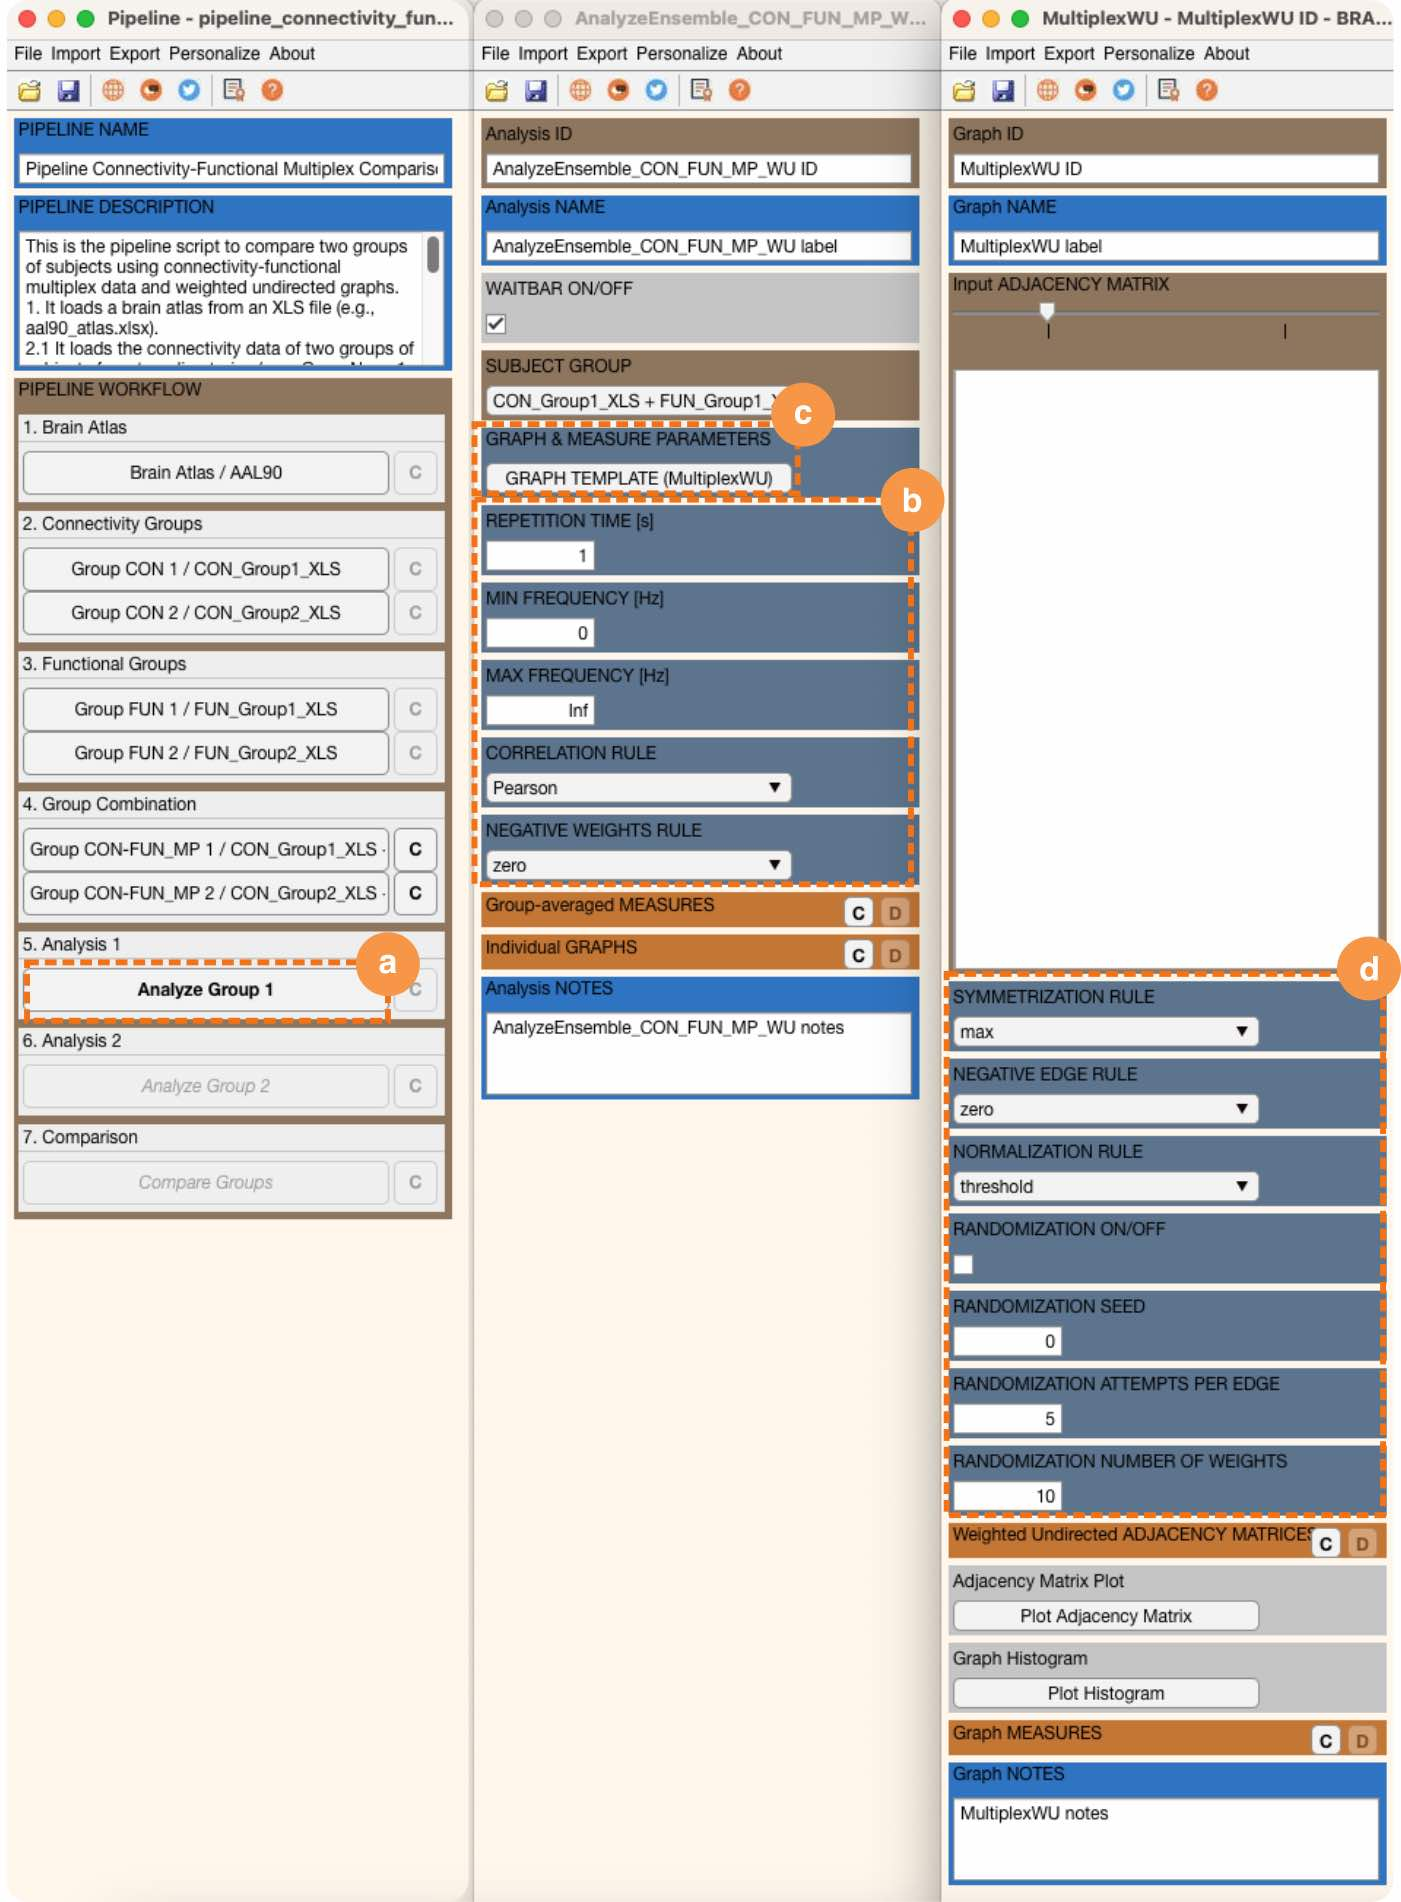
\includegraphics{fig06.jpg}
	}
	{Configuring analysis parameters}
	{
	{\bf a} To initiate the analysis of data for group 1, click on \fn{Analyze Group 1}.
 	{\bf b} In this section you can configure the analysis parameters.
 	{\bf c} By clicking on the section \code{GRAPH \& MEASURE PARAMETERS}, you open {\bf d} a new interface that permits you to configure the graph parameters.
	}
 
\subsection{Setting Graph Parameters}

To configure the graph parameters, you click on the section \code{GRAPH \& MEASURE PARAMETERS} (\Figref{fig:06}c). This will open a new interface for graph template settings. 
In brain connectivity analysis, threshold values dictate the required connection strength between different brain regions for them to be considered “connected” in a binary undirected graph. 
Adjusting these thresholds allows you to explore varying levels of brain connectivity, providing insights into how regions communicate at different threshold settings.

The available parameters are:
\begin{itemize}
	\item \code{SYMMETRIZATION RULE} determines how to symmetrize the matrix.
	\item \code{NEGATIVE EDGE RULE} determines how to remove the negative edges.
	\item \code{NORMALIZATION RULE} determines how to normalize the weights between 0 and 1.
	\item \code{THRESHOLDS} determines the thresholds. \emph{This cannot be set here. It is set in the previous step.}
	\item \code{RANDOMIZE ON/OFF} determines whether to randomize the graph. \emph{Typically not used}
	\item \code{RANDOM SEED} is the randomization seed. \emph{Typically not used}
	\item \code{RANDOMIZATION ATTEMPTS PER EDGE} is the attempts to rewire each edge. \emph{Typically not used}
\end{itemize}

\end{document}